\documentclass{bioinfo}
\copyrightyear{2015} \pubyear{2015}

\access{Advance Access Publication Date: Day Month Year}
\appnotes{Manuscript Category}

\begin{document}
\firstpage{1}

\subtitle{Subject Section}

\title[short Title]{Model Sub-tissue Morphological Components in mass spectrometry imaging data Using Dirichlet Gaussian Mixture Model}
\author[Sample \textit{et~al}.]{Corresponding Author\,$^{\text{\sfb 1,}*}$, Co-Author\,$^{\text{\sfb 2}}$ and Co-Author\,$^{\text{\sfb 2,}*}$}
\address{$^{\text{\sf 1}}$Department, Institution, City, Post Code, Country and \\
$^{\text{\sf 2}}$Department, Institution, City, Post Code,
Country.}

\corresp{$^\ast$To whom correspondence should be addressed.}

\history{Received on XXXXX; revised on XXXXX; accepted on XXXXX}

\editor{Associate Editor: XXXXXXX}

\abstract{\textbf{Motivation:} Text Text Text Text Text Text Text Text Text Text Text Text Text
Text Text Text Text Text Text Text Text Text Text Text Text Text Text Text Text Text Text Text
Text Text Text Text Text Text Text Text Text Text Text Text Text Text Text Text Text Text Text
Text Text Text Text Text Text
Text Text Text Text Text.\\
\textbf{Results:} Text  Text Text Text Text Text Text Text Text Text  Text Text Text Text Text
Text Text Text Text Text Text Text Text Text Text Text Text Text  Text Text Text Text Text Text\\
\textbf{Availability:} Text  Text Text Text Text Text Text Text Text Text  Text Text Text Text
Text Text Text Text Text Text Text Text Text Text Text Text Text Text  Text\\
\textbf{Contact:} \href{name@bio.com}{name@bio.com}\\
\textbf{Supplementary information:} Supplementary data are available at \textit{Bioinformatics}
online.}

\maketitle

\section{Introduction}


Mass spectrometry imaging (MSI) provides spatially resolved abundance information of molecules in complicated biological samples that makes MSI a powerful tool in biological and clinical research, such as biomarker discovery, metabolomics, drug delivery and cancer identification. MSI data can be considered as  an image within which each pixel has a mass spectrum containing  abundance information of a variety of molecular $m/z$s or multiple images of abundance of individual $m/z$.  Due to different organization of cell types in biological tissues,  biological tissues usually have different morphologies of different sizes and structures, which result in different chemical components.  With different functions and roles in metabolic pathway, a molecule might have homogeneous distribution across the whole tissue or heterogeneous distribution with different morphological components.  Evaluating ion of specific interest is homogeneous or heterogeneous distributed is of great importance in clinical study. For example, examination of homogeneity of delivered drug in targeted area is helpful to understand response to chemotherapy and drug resistance. Moreover, spatial information of heterogeneity could potentially be used to study interactions of molecules and relationships between molecules and biological structures.  For quantitative analysis of MSI datasets, such as comparison of individual $m/z$ abundance among different tissue cohorts or different sub-tissue structures, average intensity in regions of interest is mostly used. Analyzing of average intensities could not highlight the heterogeneity of molecular distribution, thus could not make use of spatial information in MSI data. Therefore, modeling sub-tissue morphological components in heterogeneous ion images is necessary and important.
Unfortunately, complete mining of spatial patterns in MSI data currently requires the user to click through each image and look for ion distributions that may correlate to the morphology of the sample analyzed. In recent years, spatial resolution, mass resolution and source of sample for MSI technique have been improved significantly. As a result, the size of a typical MSI data size is increased to 10 GB (Need reference). 
MSI experiment typically collects 100-10000 Da m/z, which generates almost 20000 ion images for a single tissue section. Manually mining of spatial patterns  is very laborsome and subject. \\

In this paper, we proposed a new Dirichlet Gaussian Mixture model (DGMM) which incorporates spatial dependence to model spatial heterogeneity of ion image of individual $m/z$. In this model, sub-tissue morphological components of ion image of individual $m/z$ is represented by Gaussian component and ion intensity within each morphological component is assumed to follow Gaussian distribution.  The number of Gaussian components can be either pre-specified or inferred by DGMM model. A mono Gaussian component means the ion image is homogeneous, while multiple Gaussian components means the ion image is heterogeneous. The results show that DGMM is able to infer the correct number of sub-tissue morphological components of ion image of individual $m/z$ and mean intensities of each component under certain discrimination among mean intensities of each morphological components. We also showed that the proposed model can be applied to selecting morphological specific ions, clustering $m/z$s with similar spatial patterns and morphological component-wise statistical analysis.


\section{Related work}

For mining of spatial pattern and selecting $m/z$s of interest, though manually data mining is widely used, unsupervised data processing techniques are also used in imaging laboratory. \\
\\
Peak picking from a mean spectrum can pick out highly abundant ions, while the ions co-localized in a small area may missed. Moreover, the picked high abundant ions may not have the morphological information and distributed globally homogeneous instead.\\
\\
For dimension reduction method, such as principle component analysis (PCA) and non-negative matrix factorization (NNMF), high dimensional $m/z$ features can be reduced to several dimensions and an image of low dimensional space will be generated. From the image of low dimensional space, spatial pattern of the summation of all $m/z$ features is easier to observe and investigate. Moreover, ions with high loadings are considered as "important ions". However, ions with high loadings represent globally high variance, which are not necessarily the ions which correlated to the morphology of sample.\\
\\
Multivariate segmentation methods such as spatial k-means and spatial centroid segmentation, are also popular methods to explore the similarity and spatial correlation of pixels. Spatial K-means segmentation is not able to select ions, while spatial centroid segmentation can select important ions related to each segments. However the segmentation results of these multivariate menthods can not represent every single ion spatial distribution morphology, which is shown in Figure 1 and Figure 2. Moreover, sometimes the "spatial mask" of spatial K-means and spatial centroid segmentation is difficult to interpret, as shown in Figure 2.\\
\\  

Other than the spatial pattern of the summation of all $m/z$ features, sometimes people are interested in looking at ion image of individual ion, for example: biomarker discovery and the distribution of a specific drug. To our best knowledge, there're three approaches to model single ion image quantitatively. 
One proposed a homogeneity index based on a new texture anaysis technique to evaluate the level of homogeneity of single ion distribution.
XXXX proposed structured and non-structured index, which used a new form of entropy of evaluate the level of structuredness of ion images to select low abundant but structured ions.
However, none of these methods can give further information of  the spatial morphology of single ion image when the ion image is heterogeneous.
XXXXX performed morphometric analysis on ion images of individual $m/z$ features and used information of number of objects and number of surface as addition information for classification and biomarker discovery. The drawback of this method is that the model of heterogeneity of ion distribution is binary. \\

\begin{figure}[b!]
    \centering
	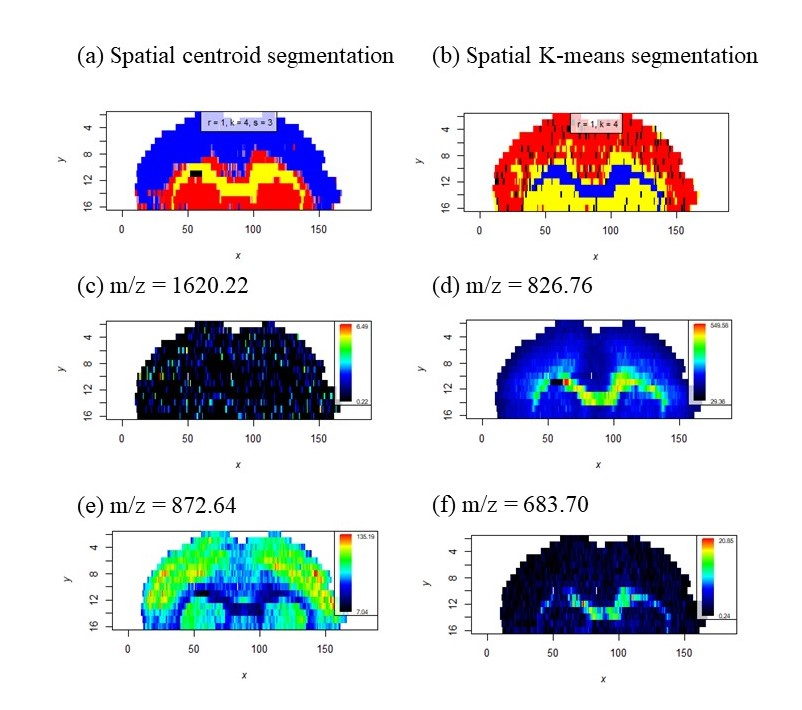
\includegraphics[width=0.4\textwidth]{figure1.jpg}
    \caption{ MSI data of a mouse brain tissue. (a) spatial centroid segmentation results of 433 $m/z$s; (b) spatial K-means segmentation results of 433 $m/z$s; (c-f) sing ion image of $m/z$ 1620.22, 826.76, 872.64 and 683.70 respectively.}
    \label{fig:figure1}
\end{figure}
\citealp{Boffelli03} might want to know about text text text
text\vspace*{1pt}





\section{Methods}
\subsection{DGMM formulas}
$x^i, i = (1,2,...,N)$, denotes the ion intensity at pixel $i$.\\
$\pi^i={\pi^i_1,..., \pi^i_K}$ denotes the prior probability of each component the $i_{th}$ pixel belongs to.\\
$z^i={z^i_1,...,z^i_K}$ denotes the discrete label of the $i_{th}$ pixel.\\
$$z^i_j=\left\{\begin{matrix}
1 \textrm{ if pixel i belongs to component j}\\ 
0 \textrm{ otherwise} 

\end{matrix}\right.$$

$$p(x^i)=\sum_{j=1}^{K}\pi^i_jp(x^i|\theta_j)$$

$$p(x^i)=\sum_{j=1}^{K}\pi^i_jp(x^i|\theta_j)p(\theta_j|\theta_{T_j})$$

$$p(x^i)=\sum_{j=1}^{K}\pi^i_jp(x^i|\theta_j)p(\theta_j|\theta_{T_j}+\gamma \theta_{T_j}')$$

$$p(x^i|\theta_j)=\frac{1}{(2\pi)^{1/2}}exp(-\frac{1}{2}(x^i-\mu_j)^2\sigma_j^{-1})$$

The log-likelihood is:

$$L(\Theta )=\sum_{i=1}^{N}log{\sum_{j=1}^{K}\pi^i_jp(x^i|\theta_j)}+logp(\Pi )$$

The discrete label $z^i_j$ is a random variable following a multinomial distribution with $M$ realizations.\\

$$p(z^i|\xi ^i)=\frac{M!}{\prod_{j=1}^{K}(z^i_j)!}\prod_{j=1}^{K}(\xi ^i_j)^{z^i_j}$$

in which $(\xi ^i_j)\ge0$ and $\sum_{j=1}^{K}\xi ^i_j=1$

The Dirichlet process id defined as:\\

$$p(\xi ^i|\alpha^i)=\frac{\Gamma (\sum_{j=1}^{K}\alpha^i_j)}{\prod_{j=1}^{K}\Gamma (\alpha^i_j)}\prod_{j=1}^{K}(\xi^i_j)^{(\alpha^i_j-1)}$$

In which, $\alpha^i (\alpha^i>0)$ is the vector of Dirichlet parameters.

$$p(z^i|\alpha^i)=\frac{M!\Gamma (\sum_{j=1}^{K}\alpha^i_j)}{\prod_{j=1}^{K}(z^i_j)!\Gamma (\sum_{j=1}^{K}(\alpha^i_j+z^i_j))}\prod_{j=1}^{K}{\frac{\Gamma(\alpha^i_j+z^i_j)}{\Gamma(\alpha^i_j)}}$$

$$\pi^i_j=p(z^i_j=1|\alpha_i)=\frac{\alpha^i_j}{\sum_{k=1}^{K}\alpha^i_k}$$

Incorporate the spatial dependence:\\

The posterior probability at iteration $t$ is given by:


$$y^{i(t)}_j=\frac{\pi^i_jp(x^i|\theta_j)}{\sum_{k=1}^{K}\pi^i_kp(x^i|\theta_k)}$$

To introduce the relationship between neighboring pixels, define\\

$$\bar{y}^{i}_j=\frac{1}{\sum_{m\subseteq N^i}d^i_m}\sum_{m\subseteq N^i}d^i_{m}y^{m(t-1)}_j$$

In which, $d^i_m$ is the combination of spatial distance and spectrum similarity of two neighboring pixels, which can be written as:\\

$$d^i_m=exp(\frac{(i-m)^2}{\sigma_1})exp(\frac{(S_i-S_m)^2}{\sigma_2})$$

The new Dirichlet distribution is defined as:\\
$$p(\xi ^i|\alpha^i)=\frac{\Gamma (\sum_{j=1}^{K}\alpha_j^2 \bar{y}^{(i)\beta}_j)}{\prod_{j=1}^{K}\Gamma (\alpha_j^2 \bar{y}^{(i)\beta}_j)}\prod_{j=1}^{K}(\xi^i_j)^{(\alpha_j^2 \bar{y}^{(i)\beta}_j-1)}$$

Therefore, the error function $E(\Theta )$ is:
$$E(\Theta )=-\sum_{i=1}^{N}\sum_{j=1}^{K}y^{i(t)}_j\{log(\alpha_j^2\bar{y}^{(i)\beta}_j)-log(\sum_{k=1}^{K}\alpha_k^2\bar{y}^{(i)\beta}_k)-\frac{1}{2}log(2\pi)-\frac{1}{2}log(\sigma_j)-\frac{1}{2}(x^i-\mu_j)^2\}$$

In which, $\Theta =(\mu_j, \sigma_j, \alpha_j, \beta)$\\

The objective is to $min_\Theta E(\Theta)$.\\


In the M step,
$$\Theta ^{(t+1)}=\Theta ^{(t)}-\eta \bigtriangledown E(\Theta ^{(t)})$$

In which $eta$ is the learning step. All $\bigtriangledown E(\Theta ^{(t)})$ has closed form and are subject to the constrains.\\
Details of differential of each parameter:
$$$$

\subsection{Framwork of data processing}

\begin{figure}[b!]

	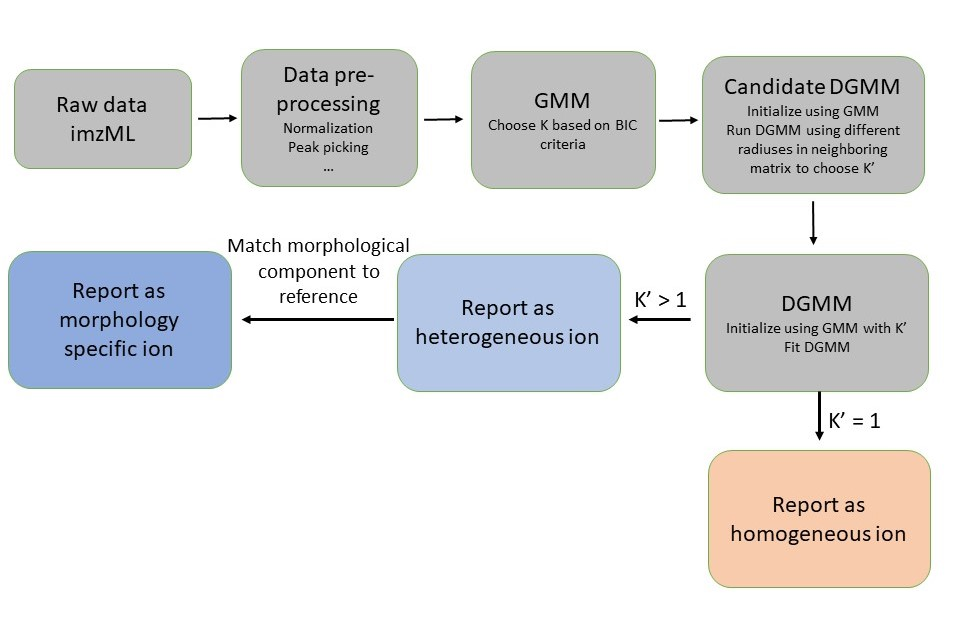
\includegraphics[width=0.5\textwidth]{figure3.jpg}
    \caption{flow chat sketch}
    \label{fig:figure3}
\end{figure}
\citealp{Boffelli03} might want to know about text text text
text\vspace*{1pt}

\begin{table}[!t]
\processtable{This is table caption\label{Tab:01}} {\begin{tabular}{@{}llll@{}}\toprule head1 &
head2 & head3 & head4\\\midrule
row1 & row1 & row1 & row1\\
row2 & row2 & row2 & row2\\
row3 & row3 & row3 & row3\\
row4 & row4 & row4 & row4\\\botrule
\end{tabular}}{This is a footnote}
\end{table}



\section{Datasets}

\subsection{Simulated Data}
We simulated MSI datasets using function as below:
$$Y_{i}=\mu_{k(i)}+ \phi_i + \epsilon_i $$
$$ \phi_i  \sim ICAR (\tau^2, W) $$
in which $Y_i$ is the intensity oof pixel $i$, $\mu_{k(i)}$ the mean intensity of sub-tissue morphological component $k$ pixel $i$ belongs to, $\phi_i$ the spatial auto-correlation term and $\epsilon_i$ the nosie of pixel $i$. $\epsilon_i$ follows inttrisinc auto-correllation with variance $tau^2$ and $W$ as neighboring matirx.




In the first dataset we simulated, all MSI images have identical morphologies but different noise levels. As shown in Fig XXXXX, All MSI have three morphological components: circle, triangle and the rest of image and the mean intensities of three morphological cmponents are 100, 225, 150 respectively. The noise level varies from 5\% of mean intensity to 32\% of mean intensity. The variance for spatial auto-correlation is 25.



The second simulated data has 40 images or m/zs in total and every 10 m/zs have identical morphologies but different mean intensities for each morphological component. As shown in Fig XXXX, m/z 1-10 have three morphological components: circle, triangle and the rest of image, m/z 11-20 have two morphological components: triangle and the rest of image, m/z 21-30 have two morphological components: circle and the rest of image and m/z 31-40  have homogeneous ion spatial distribution.

\subsection{Saline and CPG preconditioned mouse brain}
CpG is ann unmethylated oligodeoxynucleotide that has been shown to stimulate the toll-like receptor 9 and induce neuroprotection against ischemic damage. To estimate the metabolic changes on brains caused by CpG preconditioning, brain tissue sections of saline (control) and CpG preconditioned mice were collected and analyzed by nano-MSI experiment using a Thermo LTQ-orbitrap instrument via positive mode. The spatial resolution is approximately 40 $\times$ 200 $\mu$m and the mass range is 100-1500 Da. The original MSI data are in RAW format and converted to NetCDF format using Xcalibur software before read by Cardinal.
\subsection{Amyotrophic lateral sclerosis mouse brain}
Amyotrophic lateral sclerosis is a neurodegenerative disease, 20\% of which is caused by mutations of SOD1. Mice who expressing a human ALS mutation, Cu-Zm superoxide dismutase 1 become symptomatic after ~130 days. Brain tissue sections of ALS mice and their non-SOD1/YFP littermates on day 150 were collected and analyzed by MALDI-MSI experiment using a solariX 9.4 T FTICR
(Bruker Daltonics, Billerica, MA, USA) instrument via positive mode. The spatial resolution is 100 $\mu$m and the mass range is 609.44-1400 Da. MALDI-MSI data were converted to imzML format before further processing using R.













\section{Results and Discussion}
In this section, we will first evaluate the performance of the proposed method in terms of estimation accuracy using simulated datasets and examine the performance of the proposed model using ALS mouse brain dataset. Then we will discuss the potential applications of the proposed model in selecting morphological specific ions, clustering $m/z$s with similar spatial patterns and morphological component-wise statistical analysis.











\begin{figure}[b!]
    \centering
	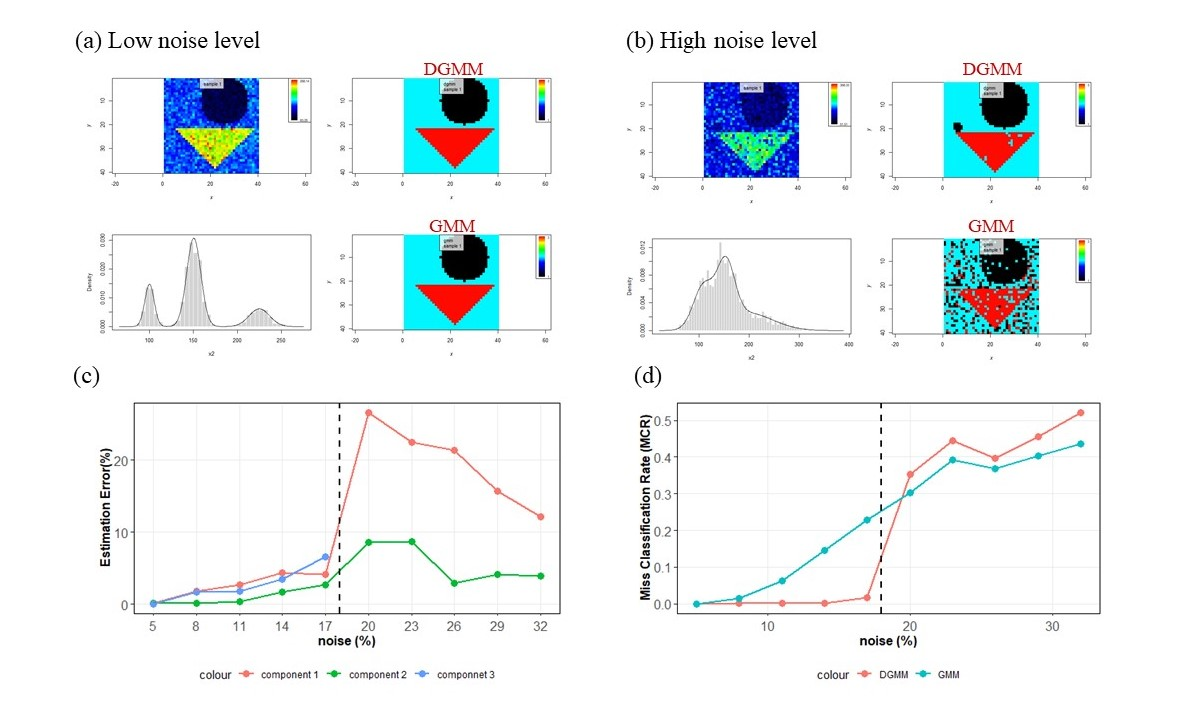
\includegraphics[width=0.6\textwidth]{figure4.jpg}
    \caption{Performance of DGMM on simulated dataset. (a) ion image (upper left), results of DGMM (upper right), histogram of ion intensities (lower left) and results of GMM(lower right) for low noise level data; (b) ion image (upper left), results of DGMM (upper right), histogram of ion itensities (lower left) and results of GMM(lower right) for high noise level data; (c) plot of estimation error of mean intensity of each morphological component vs noise level; (d) plot of misclassification rate vs noise level}
    \label{fig:figure3}
\end{figure}




\subsection{Model performance}
\subsubsection{Simulation}
As shown in Fig. \ref{fig:figure3}, for low noise level dataset, both GMM and DGMM can report the correct number of morphological components and have very low estimation error of the mean intensity of each morphological component and very low rate of misclassifying pixels to morphological components. As the noise level increases, the estimated morphological component map of ion image generated by GMM becomes very noise and the misclassification rate increases rapidly. However, the proposed model has much lower estimation error of the mean intensity of each component and misclassification rate comparing to GMM for noise level under 20\% of mean. When noise level is above 20\% of mean, the reported number of morphological components are not correct. The performance on reporting the correct number of morphological components depends on how discriminative the intensities of these components are. In general, for higher fold changes among mean intensities of components ans lower noise level, DGMM have better performance. In this case, the mean intensity of the background component,  circle component and triangle component have geometric 1.5 fold change and the noise tolerance is 20\%.\\
\subsubsection{ALS mouse brain}
The results of spatial K-means segmentation and spatial centroid segmentation of ALS mouse brain based on 60 $m/z$ features are shown in  Fig. \ref{fig:figure4}(a) and (b), respectively. The segmentation maps of these two multivariate analysis are strongly affected by the noisy $m/z$ features and do not show any patterns of ion image of $m/z$ 868.33 (Fig. \ref{fig:figure4}(c)), $m/z$ 838.63 (Fig. \ref{fig:figure4}(d)), $m/z$ 681.14 (Fig. \ref{fig:figure4}(e)), $m/z$ 896.57 (Fig. \ref{fig:figure4}(f)). As shown on the right panel in Fig. \ref{fig:figure4}(c-f), the proposed model can infer the number of morphological components and generate morphological component map of individual ion image. By visually comparing ion images in Fig. \ref{fig:figure4}(c-f) and their co-responding morphological component maps, the performance of model is reasonably good.


\begin{figure}[b!]
    \centering
	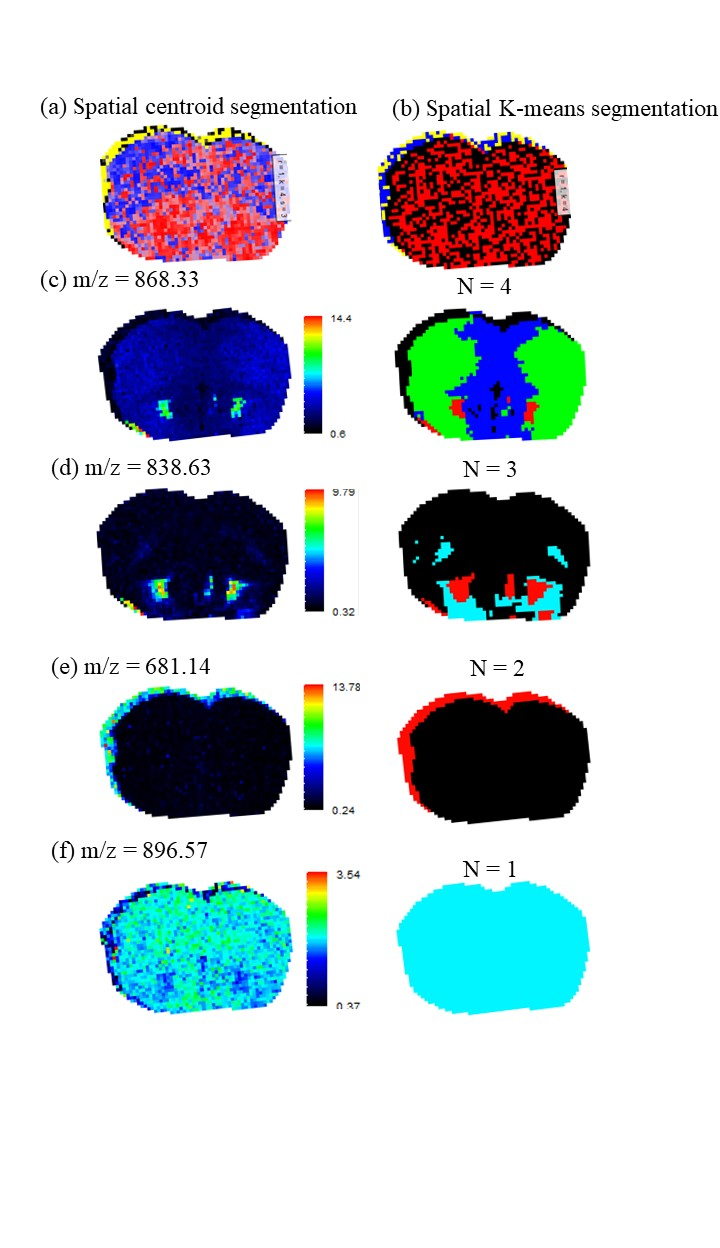
\includegraphics[width=0.4\textwidth]{long_figure.jpg}
    \caption{ MSI data of a ALS mouse brain. (a) spatial centroid segmentation results of 60 $m/z$s; (b) spatial K-means segmentation results of 60 $m/z$s; (c-f) sing ion image and corresponding morphological component map of $m/z$ 868.33, 838.63, 681.14 and 896.57 respectively.}
    \label{fig:figure4}
\end{figure}



\subsection{Select Morphological Specific Ions}
\subsubsection{Identify ion of a heterogeneous distribution or homogeneous distribution}
A critical important task in MSI data analysis is to identify $m/z$ that have a heterogeneous distribution or homogeneous distribution. $m/z$ of a heterogeneous distribution is usually related to anatomic structure of tissue or lessions, thus it's of great interest of further study. On the other hand, it's also important to evaluate whether ion has homogeneous distribution when it comes to drug delivery in clinical study. As shown in Fig. \ref{fig:figure4}, the proposed method can identify ion of a heterogeneous (Fig. \ref{fig:figure4}(f)) or homogeneous (Fig. \ref{fig:figure4}(c-e)) distribution by the number of morphological components. For $m/z$ with heterogeneous distribution, the proposed model can also provide the information of how many morphological components it has and the proportion and location of each component. (As shown in Fig. \ref{fig:figure4} (c-e)  One can customize the minimum proportion of morphological components to ignore small hot ares based on respective research goal.



\subsubsection{Identify ion having a specific morphological component}
Identifying $m/z$ of a spatial pattern related to a specific area, which can be either an anatomic structure or an area of interest, is helpful to understand the molecular signature of sub-tissue structures. Using correlation coefficient between ion image of a $m/z$ and binary matrix indicating a specific area is the most commonly used method to identify $m/z$ co-localized in this area. It's fast and reliable when the ion is only depressed or over expressed in the specific area. However when the ion has multiple morphological components, using correlation coefficient is not able to identify these $m/z$s. Fig. \ref{fig:figure6} shows that the correlation of ion image of $m/z$  844.67 is -0.51, which is comparatively low and similar to the correlation coefficient of ion image of $m/z$ 791.67. While we can see from the ion images that $m/z$  844.67 has a more clear morphology of segment showing in Fig . \ref{fig:figure6}(a). In this paper, we fit DGMM on ion images of individual $m/z$s first, then match each morphological component to the segment shown in Fig. \ref{fig:figure6}.  The morphological component of the highest matching score is considered as matched component. The morphological component of highest matching score of 0.36 in ion image of $m/z$ 791.6 is the red area. The morphological component colored in black  in ion image of $m/z$ 844.67 has the highest matching score of 0.78, which is much higher than that of the red are in ion image of $m/z$ 791.67. This example demonstrates that ion images with similar correlation may have different morphology of spatial distribution, which can be distinguished by the proposed model. 
\begin{figure}[b!]
    
	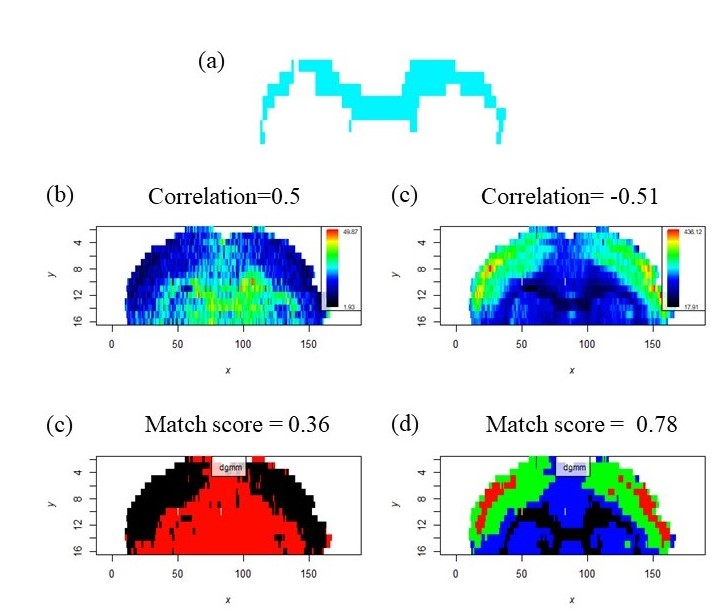
\includegraphics[width=0.5\textwidth]{figure6.jpg}
    \caption{(a) one segment generated by spatial centroid segmentation using 433 $m/z$s which looks like corpus callosum; (b) ion image of $m/z$ 791.67; (c) ion image of $m/z$  844.67; (d) morphological component map of (b) modeled by DGMM; (e) morphological component map of (c) modeled by DGMM }
    \label{fig:figure6}
\end{figure}



\subsection{Clustering $m/z$s with similar spatial patterns}


\begin{figure}[b!]
    
	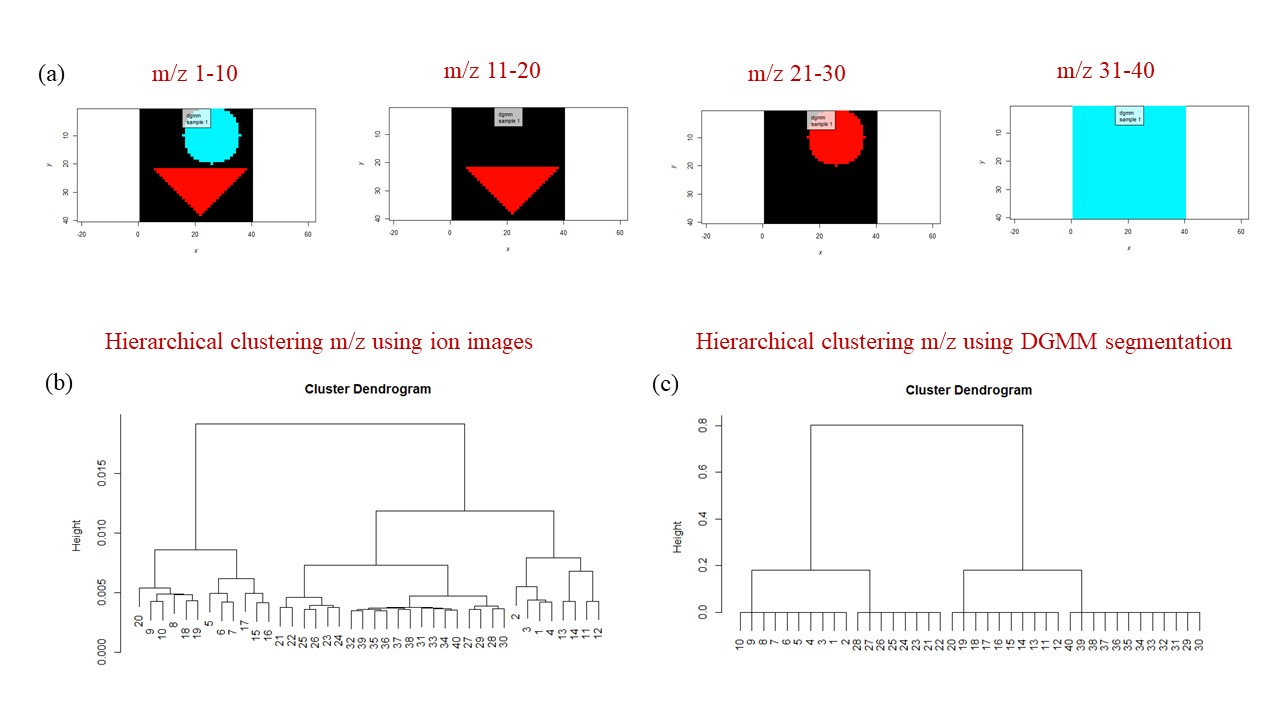
\includegraphics[width=0.8\textwidth]{figure7.jpg}
    \caption{(a) morphological components for m/z 1-10, 11-20, 21-30 and 31-40; (b) clustering $m/z$s based on ion image; (c) clustering $m/z$s based on morphological component  generated by DGMM}
    \label{fig:figure7}
\end{figure}

Grouping $m/z$s with similar spatial morphology can help understanding the interactions between $m/z$s.  A naive way of doing this is to cluster $m/z$s based on the Euclidean distance between vectors of ion images. However the spatial information will be lost and it's very sensitive to the ion intensity. In Fig. \ref{fig:figure7} (b), the simulated ion images of $m/z$ 1-10, 11-20, 21-30, 31-40 have identical spatial patterns respectively. The results of clustering based on Euclidean distance between vectors of ion images show that $m/z$s within each cluster do not have the same spatial patterns. Fig. \ref{fig:figure7} (c) shows the results of clustering $m/z$s based on the Dice distance between vectors of morphological component labels and we can see that $m/z$s within the same cluster have identical spatial patterns. Clustering $m/z$s based on their individual morphological component labels is not affected by intensities, while by spatial morphology. This provides an alternative way to study relationships between different $m/z$s.

\subsection{Morphological Component-Wise statistical analysis}


\begin{itemize}
\item problems of averaging statistical analysis
\item advantage of Morphological Component-Wise statistical analysis
\item state of concept: real data example and simulation
\end{itemize}









%%%%%%%%%%%%%%%%%%%%%%%%%%%%%%%%%%%%%%%%%%%%%%%%%%%%%%%%%%%%%%%%%%%%%%%%%%%%%%%%%%%%%
%
%     please remove the " % " symbol from \centerline{\includegraphics{fig01.eps}}
%     as it may ignore the figures.
%
%%%%%%%%%%%%%%%%%%%%%%%%%%%%%%%%%%%%%%%%%%%%%%%%%%%%%%%%%%%%%%%%%%%%%%%%%%%%%%%%%%%%%%






\section{Conclusion}

(Table~\ref{Tab:01}) Text Text Text Text Text Text  Text Text Text
Text Text Text Text Text Text  Text Text Text Text Text Text.
Figure~2\vphantom{\ref{fig:02}} shows that the above method  Text
Text Text Text  Text Text Text Text Text Text  Text Text.
\citealp{Boffelli03} might want to know about  text text text text
Text Text Text Text Text Text  Text Text Text Text Text Text Text
Text Text  Text Text Text Text Text Text.
Figure~2\vphantom{\ref{fig:02}} shows that the above method  Text
Text Text Text  Text Text Text Text Text Text  Text Text.
\citealp{Boffelli03} might want to know about  text text text text
Text Text Text Text Text Text Text Text Text Text Text Text Text
Text Text  Text Text Text Text Text Text.
Figure~2\vphantom{\ref{fig:02}} shows that the above method  Text
Text Text Text  Text Text Text Text Text Text  Text Text.



Text Text Text Text Text Text  Text Text Text Text Text Text Text
Text Text  Text Text Text Text Text Text.
Figure~2\vphantom{\ref{fig:02}} shows that the above method  Text
Text Text Text  Text Text Text Text Text Text  Text Text.
\citealp{Boffelli03} might want to know about  text text text text

\begin{enumerate}
\item this is item, use enumerate
\item this is item, use enumerate
\item this is item, use enumerate
\end{enumerate}

Text Text Text Text Text Text Text Text Text Text Text Text Text
Text Text Text Text Text Text Text Text.
Figure~2\vphantom{\ref{fig:02}} shows\vadjust{\pagebreak} that the
above method  Text Text Text Text Text Text Text Text Text Text
Text Text.  \citealp{Boffelli03} might want to know about text
text text text Text Text Text Text Text Text  Text Text Text Text
Text Text Text Text Text Text Text Text Text Text Text.
Figure~2\vphantom{\ref{fig:02}} shows that the above method  Text
Text Text Text Text Text Text Text Text Text  Text Text.
\citealp{Boffelli03} might want to know about text text text text
Text Text Text Text Text Text  Text Text Text Text Text Text Text
Text Text Text Text Text Text Text\break Text.


Text Text Text Text Text Text  Text Text Text Text Text Text Text
Text Text  Text Text Text Text Text Text.
Figure~2\vphantom{\ref{fig:02}} shows that the above method  Text
Text Text Text\vspace*{-10pt}


\section*{Acknowledgements}

Text Text Text Text Text Text  Text Text.  \citealp{Boffelli03} might want to know about  text
text text text\vspace*{-12pt}

\section*{Funding}

This work has been supported by the... Text Text  Text Text.\vspace*{-12pt}

%\bibliographystyle{natbib}
%\bibliographystyle{achemnat}
%\bibliographystyle{plainnat}
%\bibliographystyle{abbrv}
%\bibliographystyle{bioinformatics}
%
%\bibliographystyle{plain}
%
%\bibliography{Document}


\begin{thebibliography}{}

\bibitem[Bofelli {\it et~al}., 2000]{Boffelli03}
Bofelli,F., Name2, Name3 (2003) Article title, {\it Journal Name}, {\bf 199}, 133-154.

\bibitem[Bag {\it et~al}., 2001]{Bag01}
Bag,M., Name2, Name3 (2001) Article title, {\it Journal Name}, {\bf 99}, 33-54.

\bibitem[Yoo \textit{et~al}., 2003]{Yoo03}
Yoo,M.S. \textit{et~al}. (2003) Oxidative stress regulated genes
in nigral dopaminergic neurnol cell: correlation with the known
pathology in Parkinson's disease. \textit{Brain Res. Mol. Brain
Res.}, \textbf{110}(Suppl. 1), 76--84.

\bibitem[Lehmann, 1986]{Leh86}
Lehmann,E.L. (1986) Chapter title. \textit{Book Title}. Vol.~1, 2nd edn. Springer-Verlag, New York.

\bibitem[Crenshaw and Jones, 2003]{Cre03}
Crenshaw, B.,III, and Jones, W.B.,Jr (2003) The future of clinical
cancer management: one tumor, one chip. \textit{Bioinformatics},
doi:10.1093/bioinformatics/btn000.

\bibitem[Auhtor \textit{et~al}. (2000)]{Aut00}
Auhtor,A.B. \textit{et~al}. (2000) Chapter title. In Smith, A.C.
(ed.), \textit{Book Title}, 2nd edn. Publisher, Location, Vol. 1, pp.
???--???.

\bibitem[Bardet, 1920]{Bar20}
Bardet, G. (1920) Sur un syndrome d'obesite infantile avec
polydactylie et retinite pigmentaire (contribution a l'etude des
formes cliniques de l'obesite hypophysaire). PhD Thesis, name of
institution, Paris, France.

\end{thebibliography}
\end{document}
